\subsection{Benötigte Kenntnisse}
Die Variable x=0-3 dient als Index.\\
Um das Programm zu erstellen sollten Kenntnisse z.B. für die Timer CCU4x sowie deren Slices CC40-43 vorhanden sein. Die Funktionen der CCU4x wird in der Reference Manuel beschrieben, siehe dazu Anhang, um die Timer zu Initialisieren wird die XMC LIb benötigt die eine fertige API mit bringt, siehe Kapitel Besonderheiten der Software, so wird nur noch die API mit den richtigigen Parametern beschrieben um die Timer lauffähig zu kriegen. Um Fehler in der Zeitnahme zu verringern sollten Zeitwerte, die ausgelesen werden sollen direkt am Anfang des Interrupts in Variablen gespeichert werden und nicht erst innerhalb anderer Anweisungen oder Schleifen, da das schon deutliche Abweichungen mit sich bringt.\\

\subsubsection{Durchgeführte Berechnungen}
Auch für die Programmierung waren diverse Berechnungen notwendig. So zum Beispiel musste zur Erzeugung der Ultraschallimpulse ein Pulsweitenmoduliertes Rechteck signal geschaffen werden. Dafür wurde ein Timer der CCU4x auf einen Takt von 40kHz eingestellt. So musste bei einem Timertakt von 96MHz eine Periodendauer von 2400 Takten konfiguriert sein und ein Compare-Wert von 1200 Takten, siehe unten die Berechnung. Im Zählvorgang des Timers wird der Ausgang nach erreichen des Compare-Wertes auf 1 gesetzt, und nach erreichen der Periodendauer wieder auf 0 zurückgesetzt. Dadurch ergibt sich eine Periodendauer von 25us, was einer Frequenz von 40kHz entspricht.\\
Auch zur Erfassung der Zeit, die vergeht bis das Echo des Ultraschall-Impulses zurück kommt wird über einen Timer der CCU4x erfasst. 
\onehalfspacing \\ \\
\(\displaystyle Periodendauer=\frac{96MHz}{40kHz} = 2400 \)  \  \  \    \(\displaystyle Compare-Wert=\frac{2400}{2} = 1200 \) 
\singlespacing

Siehe Kapitel Messungen am Ausgang des Controller für das PWM Signal sowie die Einstellung der einzelnen Timer, Anhang PWM Configuration sowie Timer Configuration.

\subsection{Quellcodeentwurf}

\textbf{Programmstruktur:}
Anstatt alles in der main.c an ,siehe Abbildung \ref{fig:main.c1}, Programmcode zu verfassen was bei sehr komplexen Programmen schnell zu unübersichtlichkeit führt hat das Auslagern den Vorteil das der Quellcode Logisch getrennt werden kann und so einer verschlankerung des Codes mit sich bringt. 
Somit stehen in der Main  vor allem die Aufrufe der verschiedenen benötigten Funktionen. So sieht man in der Main jetzt deutlich, welche Funktionen beim Starten initialisiert werden, und welche Unterprogramme regelmäßig aufgerufen werden. Auch vereinfacht diese Struktur gerade bei Prototypen das Testen der Funktion, so kann im Falle einerfehlerhaften Funktion einfach der Aufruf auskommentiert werden um zu testen, ob der Fehler wirklich von der Funktion herrührt. Dadurch müssen nicht etliche Zeilen Programmcode der Funktion auskommentiert werden, wodurch schnell Fehler entstehen könnten, durch übriggebliebene Zeichen, oder gar beim entfernen der Auskommentierung gelöschte Zeichen.\\
\begin{minipage}{1\textwidth}
\begin{lstlisting}
#include <stdio.h>
#include <stdbool.h>
#include "bricklib2/logging/logging.h"
#include "bricklib2/bootloader/bootloader.h"
#include "communication.h"
/****Eigene Include Dateien*******/
#include "configs/config.h"
#include "system_timer/system_timer.h"
#include "a16pt.h"
int main(void)
{ 
	logging_init(); 
	logd("Start Distance US V2 Bricklet/n/r");  	//For the Debugmodus
	communication_init(); 					//Function call
	a16pt_init(); 								//Function call	
	while(true)
	{
		a16pt_tick(); 						//Function call
		bootloader_tick(); 					//Function call
		communication_tick(); 				//Function call
		
	}
}
\end{lstlisting}
\captionof{figure}{main.c}
\label{fig:main.c1}
\end{minipage}\\
Um die Function call zu verstehen muss die Abbildung \ref{fig:a16pt.h}: a16pt.h näher betrachtet werden.
In der der a16pt.h werden die Funktionen definiert die dann in der main.c aufgerufen werden und die Funktionsanweisungen stehen dafür in der a16pt.c. \ref{fig:a16pt.c}\\
\begin{minipage}{1\textwidth}
\begin{lstlisting}
#ifndef A16PT_H
#define A16PT_H
#include <stdint.h>
void a16pt_init(void);				//Functional definition
void a16pt_tick(void); 			//Functional definition
uint16_t a16pt_get_distance(void); //Functional definition
#endif
\end{lstlisting}
\captionof{figure}{a16pt.h}
\label{fig:a16pt.h}
\end{minipage}\\
\\
\textbf{Init Aufruf:}
Auch in der \ref{fig:a16pt.c} a16pt.c Init gibt es weitere Funktionsaufrufe wo z.B. die PWM oder der Externe Interrupt Initialisiert werden.

\begin{minipage}{1\textwidth}
\begin{lstlisting}
void a16pt_init(void)
{

/*****************Externe_Interrupt*******************/

	eru_init(eru_port);

/************PWM_Init*****************************/

	XMC_CCU4_Init(CCU41, XMC_CCU4_SLICE_MCMS_ACTION_TRANSFER_PR_CR_PCMP);
	XMC_CCU4_StartPrescaler(CCU41);

	ccu4_pwm_init(pwm_port_0,cc40, period_1);	//P4_4
	ccu4_pwm_set_duty_cycle( cc40, compare_1);

	ccu4_pwm_init(pwm_port_1,cc42, period_0);	//P4_6
	ccu4_pwm_set_duty_cycle( cc42, compare_0);
.
.
.
.
\end{lstlisting}
\captionof{figure}{Ein Teilausschnitt von der a16pt.c Init Aufruf }
\label{fig:a16pt.c}
\end{minipage}



\textbf{Interrupt Aufruf:}
In der Abbildung \ref{fig:a16pt.c1} :a16pt.c Interrupt Aufruf, werden die für die Entfernungsmessung notwendigen Funktionen und die Interrupt anweisungen, in dem Fall die IRQ21, abgearbeitet außerdem werden die Timer Synchron abgeschaltet und aus experementellen gründen wurde ein weitere Impuls generiert um zu beobachten wie sich das nachschwingen verhält bei einer längeren Kurzschlusszeit an der Ultraschallkapsell. 
\\
\begin{minipage}{1\textwidth}
\begin{lstlisting}

/*************Interrupt_Funktionen****************/

void IRQ_Hdlr_21(void) // Compare Interrupt counter 10
{

	// Disable IRQs so we can't be interrupted
	__disable_irq();

	// Set CCU trigger to low, otherwise ccu counter is restarted
	XMC_SCU_SetCcuTriggerLow(XMC_SCU_CCU_TRIGGER_CCU41);

	// Stop slice 2
	XMC_CCU4_SLICE_StopClearTimer(CCU41_CC40);

	// For slice 1 we wait until PWM is run through (to get exactly 10 pwm peaks on P4_4 and P4_6)
	while(XMC_CCU4_SLICE_GetTimerValue(CCU41_CC42) > compare_1) {

		__NOP();
	}
	
	//new pin configuration
	const XMC_GPIO_CONFIG_t pin_out_config	= {
			.mode                = XMC_GPIO_MODE_OUTPUT_PUSH_PULL,
			.output_level        = XMC_GPIO_OUTPUT_LEVEL_HIGH,
		};

	 XMC_GPIO_Init(P4_6, &pin_out_config);
	//Creat a high impulse
	for(s=0; s<50; s++)
		{
			__NOP();
		}
	// Stop slice 0
	XMC_CCU4_SLICE_StopClearTimer(CCU41_CC42);
	
	//pin configuration back to the PWM-Mode
	const XMC_GPIO_CONFIG_t gpio_out_config1	= {
		.mode                = XMC_GPIO_MODE_OUTPUT_PUSH_PULL_ALT9,
		.input_hysteresis    = XMC_GPIO_INPUT_HYSTERESIS_STANDARD,
		.output_level        = XMC_GPIO_OUTPUT_LEVEL_LOW,
	};

	XMC_GPIO_Init(P4_6, &gpio_out_config1);
	// Enable IRQs again
	__enable_irq();


}
\end{lstlisting}
\captionof{figure}{a16pt.c Interrupt Aufruf}
\label{fig:a16pt.c1}
\end{minipage}

%\newpage
%\begin{minipage}{1\textwidth}Eventuell wo anders hin
%\begin{struktogramm}(120,75)
%\forever
%\assign{\#include aufrufe}
%\while[8]{int main (void)}
 %\sub{Logging init()}
 %\sub{logd ("start Distance us v2 Bricklet")}
 %\sub{Communication init()}
 %\sub{a16pt init()}
%\while[8]{while (1)}
 %\sub{a16pt\_tick()}
 %\sub{bootloader\_tick()}
% \sub{Communication\_tick()}
%\whileend
%\whileend
%\foreverend

%  \ifthenelse{10}{4}{Bedingung 1}{ja}{nein}
%    \ifthenelse{6}{6}{Bedingung 2}{ja}{nein}
%      \assign{Anweisungsblock 1}
%    \change
%      \assign{Anweisungsblock 2}
%    \ifend
%  \change
%    \assign{Anweisungsblock 3}
%  \ifend
%\sub{bla}
%\end{struktogramm}
%\captionof{figure}{Struktogramm der main}\label{fig:Struktogramm der main}
%\end{minipage}

%\newpage
%\begin{figure}[H]
%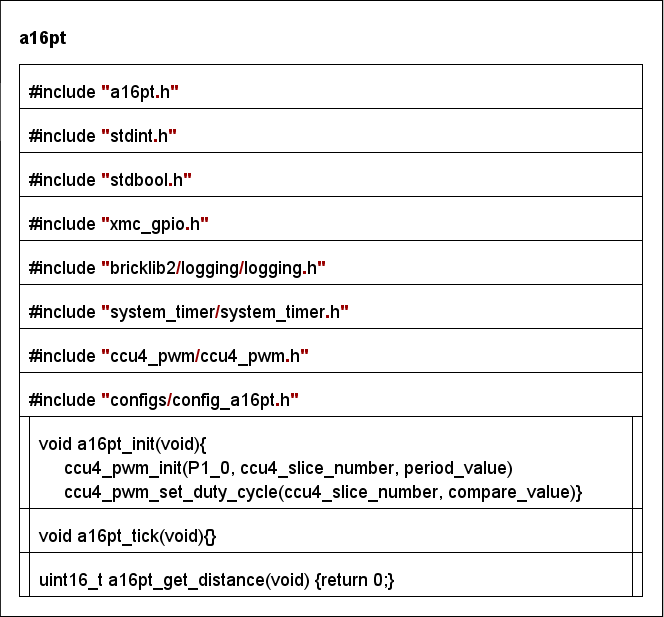
\includegraphics[width=1.0\textwidth]{Struktogramme/a16pt.png}\caption{Struktogramm der a16.pt}\label{fig:Bild2}
%\end{figure}


